% Created 2020-07-29 mer. 15:27
% Intended LaTeX compiler: pdflatex
\documentclass[t, minted]{clean-beamer}
\usepackage[utf8]{inputenc}
\usepackage[T1]{fontenc}
\usepackage{graphicx}
\usepackage{grffile}
\usepackage{longtable}
\usepackage{wrapfig}
\usepackage{rotating}
\usepackage[normalem]{ulem}
\usepackage{amsmath}
\usepackage{textcomp}
\usepackage{amssymb}
\usepackage{capt-of}
\usepackage{hyperref}
\usepackage[most]{tcolorbox}
\usepackage{bm}
\usepackage{booktabs}
\usepackage{tabularx}
\usepackage{array}
\usepackage{siunitx}
\usepackage{tikz}
\usetikzlibrary{decorations.text}
\author[shortname]{Thomas Dehaeze \inst{1,3} \and Christophe Collette \inst{1,2}}
\institute[shortinst]{\inst{1} Precision Mechatronics Laboratory, University of Liege, Belgium \and %
\inst{2} BEAMS Department, Free University of Brussels, Belgium \and %
\inst{3} European Synchrotron Radiation Facility, Grenoble, France}
\titlegraphic{\includegraphics[height=1.5cm]{figs/logo_pml.png} \hspace{5em} %
\includegraphics[height=1.5cm]{figs/logo_esrf.png} \hspace{5em} %
\includegraphics[height=1.5cm]{figs/logo_isma.png}}
\beamertemplatenavigationsymbolsempty
\addtobeamertemplate{navigation symbols}{}{%
\usebeamerfont{footline}%
\usebeamercolor[fg]{footline}%
\hspace{1em}%
\insertframenumber/\inserttotalframenumber
}
\setbeamertemplate{itemize items}[circle]
\usefonttheme[onlymath]{serif}
\AtBeginSection[]{
\begin{frame}<beamer>{Outline}
\tableofcontents[currentsection, hideothersubsections, sectionstyle=show/shaded]
\end{frame}
}
\usetheme{default}
\date{}
\title{Active Damping of Rotating Platforms using Integral Force Feedback}
\subtitle{ISMA-USD 2020, September 7-9, 2020}
\hypersetup{
 pdfauthor={},
 pdftitle={Active Damping of Rotating Platforms using Integral Force Feedback},
 pdfkeywords={},
 pdfsubject={},
 pdfcreator={Emacs 27.0.91 (Org mode 9.4)}, 
 pdflang={English}}
\begin{document}

\maketitle
\begin{frame}{Outline}
\tableofcontents
\end{frame}


\section{Dynamics of Rotating Positioning Platforms}
\label{sec:orge7d05a8}
\begin{frame}[label={sec:orgb466daa}]{Model of a Rotating Positioning Platform}
\begin{columns}
\begin{column}{0.55\columnwidth}
\begin{figure}[htbp]
\centering
\includegraphics[width=\linewidth]{figs/system.pdf}
\caption{Schematic of the studied System}
\end{figure}
\end{column}

\begin{column}{0.45\columnwidth}
Simplest model to study the \textbf{gyroscopic effects} on Decentralized IFF

\vspace{1em}

Assumptions:
\begin{itemize}
\item Perfect Rotating Stage
\item \(\dot{\theta}(t) = \Omega = \text{cst}\)
\item Small displacements
\item Position of the mass described by \([d_u\ d_v]\)
\end{itemize}

\vspace{1em}

Two frames:
\begin{itemize}
\item Inertial frame \((\vec{i}_x, \vec{i}_y, \vec{i}_z)\)
\item Uniform rotating frame \((\vec{i}_u, \vec{i}_v, \vec{i}_w)\)
\end{itemize}
\end{column}
\end{columns}
\end{frame}

\begin{frame}[label={sec:orgc029b67}]{Equations of Motion - Lagrangian Formalism}
\vspace{-1em}
\begin{equation*}
  \frac{d}{dt} \left( \frac{\partial L}{\partial \dot{q}_i} \right) + \frac{\partial D}{\partial \dot{q}_i} - \frac{\partial L}{\partial q_i} = Q_i
\end{equation*}
with \(L = T - V\) the Lagrangian, \(D\) the dissipation function, and \(Q_i\) the generalized force associated with the generalized variable.
\begin{align*}
  T &= \frac{1}{2} m \left( \left( \dot{d}_u - \Omega d_v \right)^2 + \left( \dot{d}_v + \Omega d_u \right)^2 \right), \quad V = \frac{1}{2} k \left( {d_u}^2 + {d_v}^2 \right) \\
  D &= \frac{1}{2} c \left( \dot{d}_u{}^2 + \dot{d}_v{}^2 \right), \quad Q_1 = F_u, \quad Q_2 = F_v
\end{align*}
\vspace{-1em}
\begin{align*}
  m \ddot{d}_u + c \dot{d}_u + ( k - m \Omega^2 ) d_u &= F_u + 2 m \Omega \dot{d}_v \\
  m \ddot{d}_v + c \dot{d}_v + ( k \underbrace{-\,m \Omega^2}_{\text{Centrif.}} ) d_v &= F_v \underbrace{-\,2 m \Omega \dot{d}_u}_{\text{Coriolis}}
\end{align*}
\begin{cbox}[]{blue}{}
\begin{center}
Centrifugal forces \(\Longleftrightarrow\) Negative Stiffness

Coriolis Forces \(\Longleftrightarrow\) Coupling
\end{center}
\end{cbox}
\end{frame}

\begin{frame}[label={sec:org9fc6840}]{Transfer Function Matrix the Laplace domain}
\vspace{-1em}
\begin{equation*}
  {\scriptsize \begin{bmatrix} d_u \\ d_v \end{bmatrix} = \bm{G}_d \begin{bmatrix} F_u \\ F_v \end{bmatrix}}
\end{equation*}
\begin{equation*}
  {\scriptsize \bm{G}_{d} =
               \frac{1}{k}
               \begin{bmatrix}
                 \frac{\frac{s^2}{{\omega_0}^2} + 2 \xi \frac{s}{\omega_0} + 1 - \frac{{\Omega}^2}{{\omega_0}^2}}{\left( \frac{s^2}{{\omega_0}^2} + 2 \xi \frac{s}{\omega_0} + 1 - \frac{{\Omega}^2}{{\omega_0}^2} \right)^2 + \left( 2 \frac{\Omega}{\omega_0} \frac{s}{\omega_0} \right)^2} & \frac{2 \frac{\Omega}{\omega_0} \frac{s}{\omega_0}}{\left( \frac{s^2}{{\omega_0}^2} + 2 \xi \frac{s}{\omega_0} + 1 - \frac{{\Omega}^2}{{\omega_0}^2} \right)^2 + \left( 2 \frac{\Omega}{\omega_0} \frac{s}{\omega_0} \right)^2} \\
                 \frac{- 2 \frac{\Omega}{\omega_0} \frac{s}{\omega_0}}{\left( \frac{s^2}{{\omega_0}^2} + 2 \xi \frac{s}{\omega_0} + 1 - \frac{{\Omega}^2}{{\omega_0}^2} \right)^2 + \left( 2 \frac{\Omega}{\omega_0} \frac{s}{\omega_0} \right)^2} & \frac{\frac{s^2}{{\omega_0}^2} + 2 \xi \frac{s}{\omega_0} + 1 - \frac{{\Omega}^2}{{\omega_0}^2}}{\left( \frac{s^2}{{\omega_0}^2} + 2 \xi \frac{s}{\omega_0} + 1 - \frac{{\Omega}^2}{{\omega_0}^2} \right)^2 + \left( 2 \frac{\Omega}{\omega_0} \frac{s}{\omega_0} \right)^2}
               \end{bmatrix}}
\end{equation*}

\begin{figure}[htbp]
\begin{subfigure}[c]{0.4\linewidth}
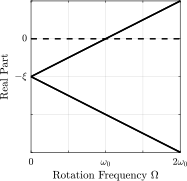
\includegraphics[width=\linewidth]{figs/campbell_diagram_real.pdf}
\caption{\label{fig:campbell_diagram_real} Real Part}
\end{subfigure}
\hfill
\begin{subfigure}[c]{0.4\linewidth}
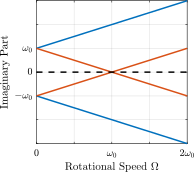
\includegraphics[width=\linewidth]{figs/campbell_diagram_imag.pdf}
\caption{\label{fig:campbell_diagram_imag} Imaginary Part}
\end{subfigure}
\hfill
\caption{Campbell Diagram : Evolution of the complex and real parts of the system's poles as a function of the rotational speed \(\Omega\)}
\centering
\end{figure}
\end{frame}

\begin{frame}[label={sec:orge87dc7b}]{Bode Plots of the System's Dynamics}
\begin{figure}[htbp]
\begin{subfigure}[c]{0.45\linewidth}
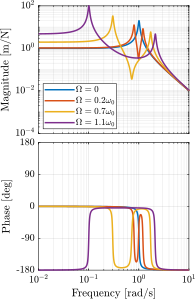
\includegraphics[width=\linewidth]{figs/plant_compare_rotating_speed_direct.pdf}
\caption{\label{fig:plant_compare_rotating_speed_direct} Direct Terms \(d_u/F_u\), \(d_v/F_v\)}
\end{subfigure}
\hfill
\begin{subfigure}[c]{0.45\linewidth}
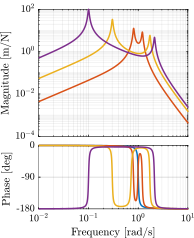
\includegraphics[width=\linewidth]{figs/plant_compare_rotating_speed_coupling.pdf}
\caption{\label{fig:plant_compare_rotating_speed_coupling} Coupling Terms \(d_v/F_u\), \(-d_u/F_v\)}
\end{subfigure}
\hfill
\caption{Bode Plots for \(\bm{G}_d\) for several rotational speed \(\Omega\)}
\centering
\end{figure}

For all the numerical analysis, \(\omega_0 = \SI{1}{\radian\per\second}\), \(k = \SI{1}{\newton\per\meter}\) and \(\xi = 0.025 = \SI{2.5}{\percent}\).
\end{frame}

\section{Problem with the Decentralized Integral Force Feedback}
\label{sec:org59c3dbc}
\begin{frame}[label={sec:org6faf2d3}]{Force Sensors and Control Architecture}
\vspace{-1em}
\begin{columns}
\begin{column}{0.6\columnwidth}
\begin{figure}[htbp]
\centering
\includegraphics[width=\linewidth]{figs/system_iff.pdf}
\caption{System with added Force Sensor in series with the actuators}
\end{figure}
\end{column}

\begin{column}{0.4\columnwidth}
\begin{figure}[htbp]
\centering
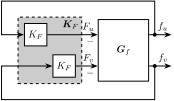
\includegraphics[width=\linewidth]{figs/control_diagram_iff.pdf}
\caption{Control Diagram for decentralized IFF}
\end{figure}

\begin{equation*}
  \bm{K}_F(s) = \begin{bmatrix} K_F(s) & 0 \\ 0 & K_F(s) \end{bmatrix}
\end{equation*}

\begin{equation*}
  K_F(s) = g \cdot \frac{1}{s}
\end{equation*}
\end{column}
\end{columns}
\end{frame}

\begin{frame}[label={sec:org387ca99}]{Plant Dynamics}
\vspace{-1em}

\begin{equation*}
  \begin{bmatrix} f_{u} \\ f_{v} \end{bmatrix} =
  \begin{bmatrix} F_u \\ F_v \end{bmatrix} - (c s + k)
  \begin{bmatrix} d_u \\ d_v \end{bmatrix}
\end{equation*}

\begin{figure}[htbp]
\centering
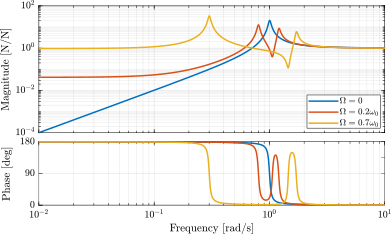
\includegraphics[width=0.9\linewidth]{figs/plant_iff_compare_rotating_speed.pdf}
\caption{Bode plot of the diagonal terms of \(\bm{G}_f\) for several rotational speeds \(\Omega\)}
\end{figure}
\end{frame}

\begin{frame}[label={sec:orgb8d521c}]{Decentralized IFF with Pure Integrators}
\begin{figure}[htbp]
\centering
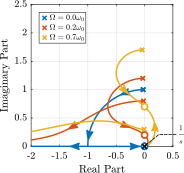
\includegraphics[width=0.7\linewidth]{figs/root_locus_pure_iff.pdf}
\caption{Root Locus for Decentralized IFF for several rotating speeds \(\Omega\)}
\end{figure}

\vspace{-1em}

\begin{cbox}[]{blue}{}
\centering For \(\Omega > 0\), the closed loop system is unstable
\end{cbox}
\end{frame}

\section{Modification of the control law: Add High-Pass Filter}
\label{sec:orgc733c30}
\begin{frame}[label={sec:orga459f5e}]{Modification of the Control Low}
\vspace{-1em}

\begin{equation*}
  K_{F}(s) = g \cdot \frac{1}{s} \cdot \underbrace{\frac{s/\omega_i}{1 + s/\omega_i}}_{\text{HPF}} = g \cdot \frac{1}{s + \omega_i}
\end{equation*}

\begin{minipage}[b]{0.45\linewidth}
\begin{center}
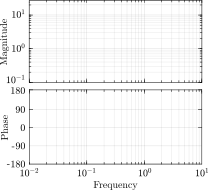
\includegraphics[width=\linewidth]{figs/loop_gain_modified_iff.pdf}
\captionof{figure}{Loop Gain}
\end{center}
\end{minipage}
\hfill
\begin{minipage}[b]{0.5\linewidth}
\begin{center}
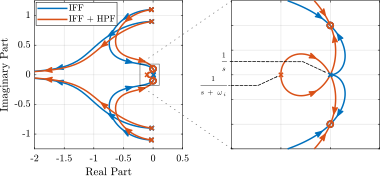
\includegraphics[width=\linewidth]{figs/root_locus_modified_iff.pdf}
\captionof{figure}{Root Locus}
\end{center}
\end{minipage}

\vspace{-1em}

\begin{align*}
\text{Added HPF} &\Longleftrightarrow \text{limit the low frequency gain} \\
                 &\Longleftrightarrow \text{shift the pole to the left along the real axis} \\
                 &\Longrightarrow \text{stable system for small values of the gain}
\end{align*}
\end{frame}


\begin{frame}[label={sec:org4390eac}]{Effect of \(\omega_i\) on the attainable damping}
\begin{figure}[htbp]
\centering
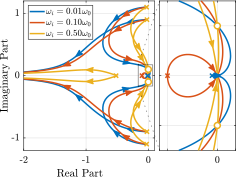
\includegraphics[width=\linewidth]{figs/root_locus_wi_modified_iff.pdf}
\caption{Root Locus for several HPF cut-off frequencies \(\omega_i\), \(\Omega = 0.1 \omega_0\)}
\end{figure}

\vspace{-2em}

\begin{columns}
\begin{column}{0.3\columnwidth}
\begin{equation*}
  g_{\text{max}} = \omega_i \left( \frac{{\omega_0}^2}{\Omega^2} - 1 \right)
\end{equation*}
\end{column}

\begin{column}{0.7\columnwidth}
\begin{cbox}[]{blue}{}
small \(\omega_i\) \(\Longrightarrow\) increase maximum damping

small \(\omega_i\) \(\Longrightarrow\) reduces maximum gain \(g_\text{max}\)
\end{cbox}
\end{column}
\end{columns}
\end{frame}

\begin{frame}[label={sec:org84c72de}]{Optimal Control Parameters}
\vspace{1em}

\begin{figure}[htbp]
\centering
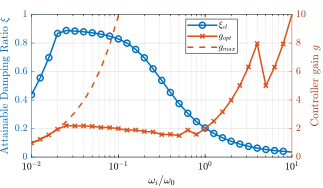
\includegraphics[width=\linewidth]{figs/mod_iff_damping_wi.pdf}
\caption{Attainable damping ratio \(\xi_\text{cl}\) as a function of the ratio \(\omega_i/\omega_0\). Corresponding control gain \(g_\text{opt}\) and \(g_\text{max}\) are also shown}
\end{figure}
\end{frame}

\section{Modification of the Mechanical System: Parallel Stiffness}
\label{sec:orgfa77c9b}
\begin{frame}[label={sec:org4d07a64}]{Stiffness in Parallel with the Force Sensor}
\vspace{-1em}
\begin{columns}
\begin{column}{0.6\columnwidth}
\begin{figure}[htbp]
\centering
\includegraphics[width=\linewidth]{figs/system_parallel_springs.pdf}
\caption{Studied system with additional springs in parallel with the actuators and force sensors}
\end{figure}
\end{column}

\begin{column}{0.4\columnwidth}
\begin{cbox}[Intuitive Idea]{blue}{}
\(k_p\) is used to counteract the negative stiffness \(-m\Omega^2\) when high control gains are used.
\end{cbox}

\vspace{-2em}

\begin{align*}
  k_p &= \alpha k \\
  k_a &= (1 - \alpha) k
\end{align*}
with \(0 < \alpha < 1\).

\vspace{1em}

The overall stiffness \(k = k_a + k_p = \text{cst}\) \(\Longrightarrow\) the open-loop poles remains unchanged
\end{column}
\end{columns}
\end{frame}

\begin{frame}[label={sec:org223db59}]{Effect of the Parallel Stiffness on the Plant Dynamics}
\begin{minipage}[b]{0.42\linewidth}
\begin{figure}[htbp]
\centering
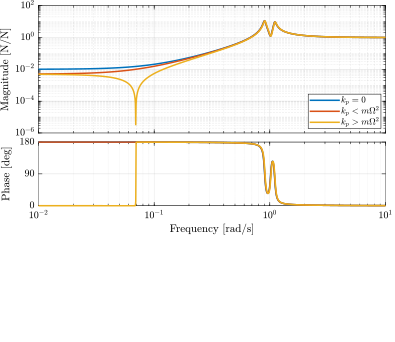
\includegraphics[width=\linewidth]{figs/plant_iff_kp.pdf}
\caption{Bode Plot of \(f_u/F_u\) for \(k_p = 0\), \(k_p < m \Omega^2\) and \(k_p > m \Omega^2\), \(\Omega = 0.1 \omega_0\)}
\end{figure}
\end{minipage}
\hfill
\begin{minipage}[b]{0.55\linewidth}
\begin{figure}[htbp]
\centering
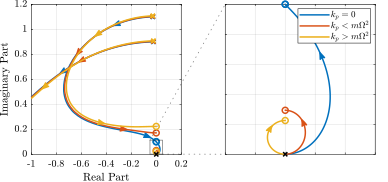
\includegraphics[width=\linewidth]{figs/root_locus_iff_kp.pdf}
\caption{Root Locus for IFF without parallel spring, with parallel springs with stiffness \(k_p < m \Omega^2\) and \(k_p > m \Omega^2\), \(\Omega = 0.1 \omega_0\)}
\end{figure}
\end{minipage}

\begin{cbox}[]{blue}{}
If \(k_p > m \Omega^2\), the poles of the closed-loop system stay in the (stable) right half-plane, and hence the \textbf{unconditional stability of IFF is recovered}.
\end{cbox}
\end{frame}

\begin{frame}[label={sec:org8be51fd}]{Optimal Parallel Stiffness}
\begin{figure}[htbp]
\begin{subfigure}[c]{0.49\linewidth}
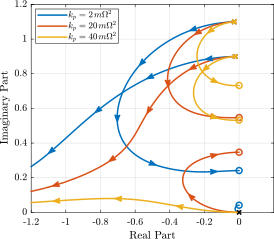
\includegraphics[width=\linewidth]{figs/root_locus_iff_kps.pdf}
\caption{\label{fig:root_locus_iff_kps} Comparison of three parallel stiffnesses \(k_p\)}
\end{subfigure}
\hfill
\begin{subfigure}[c]{0.49\linewidth}
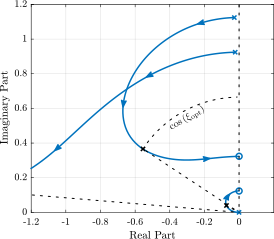
\includegraphics[width=\linewidth]{figs/root_locus_opt_gain_iff_kp.pdf}
\caption{\label{fig:root_locus_opt_gain_iff_kp} \(k_p = 5 m \Omega^2\), optimal damping \(\xi_\text{opt}\) is shown}
\end{subfigure}
\hfill
\caption{Root Locus for IFF when parallel stiffness \(k_p\) is added, \(\Omega = 0.1 \omega_0\)}
\centering
\end{figure}

\begin{cbox}[]{blue}{}
\centering
Large parallel stiffness \(k_p\) reduces the attainable damping.
\end{cbox}
\end{frame}

\section{Comparison of the two Proposed Modifications}
\label{sec:orge227508}
\begin{frame}[label={sec:org783f2c4}]{Comparison of the Attainable Damping}
\begin{figure}[htbp]
\centering
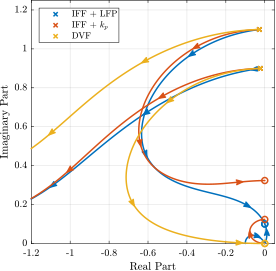
\includegraphics[width=0.7\linewidth]{figs/comp_root_locus.pdf}
\caption{Root Locus for the two proposed modifications of decentralized IFF, \(\Omega = 0.1 \omega_0\)}
\end{figure}
\end{frame}

\begin{frame}[label={sec:orgdd42828}]{Comparison Transmissibility and Compliance}
\begin{figure}[htbp]
\begin{subfigure}[c]{0.49\linewidth}
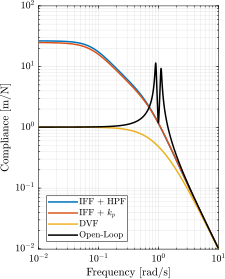
\includegraphics[width=\linewidth]{figs/comp_compliance.pdf}
\caption{\label{fig:comp_compliance} Compliance}
\end{subfigure}
\hfill
\begin{subfigure}[c]{0.49\linewidth}
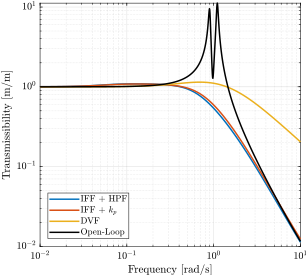
\includegraphics[width=\linewidth]{figs/comp_transmissibility.pdf}
\caption{\label{fig:comp_transmissibility} Transmissibility}
\end{subfigure}
\hfill
\caption{Comparison of the two proposed Active Damping Techniques, \(\Omega = 0.1 \omega_0\)}
\centering
\end{figure}
\end{frame}

\begin{frame}[label={sec:org5db221d}]{Conclusion \& Further work}
The two proposed techniques gives almost identical results but are very different when it comes to their implementations

\vspace{2em}

The best technique depends on the application

\vspace{2em}

\begin{wrapfigure}{r}{0.45\textwidth}
\vspace{-1em}
\begin{center}
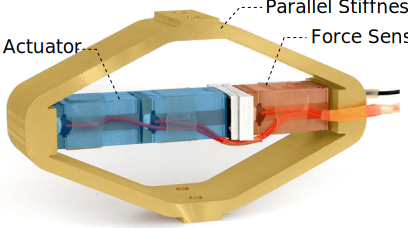
\includegraphics[width=\linewidth]{figs/apa_schematic.pdf}
\end{center}
\end{wrapfigure}

Amplified Piezoelectric Actuators are a nice way to have an actuator, a force sensors and a parallel stiffness in a compact manner

\vspace{2em}

Will be tested on the nano-hexapod
\end{frame}
\end{document}
